\documentclass[12pt]{article}
\setlength\parindent{0pt}
\usepackage{fullpage}
\usepackage{graphicx}
\usepackage{amsmath}
\setlength{\parskip}{4mm}
\def\LL{\left\langle}   % left angle bracket
\def\RR{\right\rangle}  % right angle bracket
\def\LP{\left(}         % left parenthesis
\def\RP{\right)}        % right parenthesis
\def\LB{\left\{}        % left curly bracket
\def\RB{\right\}}       % right curly bracket
\def\PAR#1#2{ {{\partial #1}\over{\partial #2}} }
\def\PARTWO#1#2{ {{\partial^2 #1}\over{\partial #2}^2} }
\def\PARTWOMIX#1#2#3{ {{\partial^2 #1}\over{\partial #2 \partial #3}} }
\newcommand{\BE}{\begin{displaymath}}
\newcommand{\EE}{\end{displaymath}}
\newcommand{\BNE}{\begin{equation}}
\newcommand{\ENE}{\end{equation}}
\newcommand{\BEA}{\begin{eqnarray}}
\newcommand{\EEA}{\nonumber\end{eqnarray}}
\newcommand{\EL}{\nonumber\\}
\newcommand{\la}[1]{\label{#1}}
\newcommand{\ie}{{\em i.e.\ }}
\newcommand{\eg}{{\em e.\,g.\ }}
\newcommand{\cf}{cf.\ }
\newcommand{\etc}{etc.\ }
\newcommand{\Tr}{{\rm tr}}
\newcommand{\etal}{{\it et al.}}
\newcommand{\OL}[1]{\overline{#1}\ } % overline
\newcommand{\OLL}[1]{\overline{\overline{#1}}\ } % double overline
\newcommand{\OON}{\frac{1}{N}} % "one over N"
\newcommand{\OOX}[1]{\frac{1}{#1}} % "one over X"



\begin{document}
\Large
\centerline{\sc{Homework 6}}
\normalsize
\centerline{\sc{Due Friday, 31 March}}

\begin{enumerate}

  \item{We saw in class that in a pendulum the string does no work. We also saw that the normal force does no work on an object sliding down a ramp.}
    \begin{enumerate}
      \item{Explain why the tension in the string of a pendulum does no work.}
      \item{Explain why the normal force does no work on an object sliding down a ramp.}
      \item{Give an example of a situation where tension {\it does} do work on an object.}
      \item{Give an example of a situation where friction does positive work on something.}
    \end{enumerate}

\item On a cold winter day, you might rub your hands together to warm them up. The kinetic friction as you rub your hands together does negative work on your hands.
The law of conservation of energy (which we will study in more detail next week) says that energy is never lost, only converted from one form to another; in this case,
this energy is dissipated as heat. 
\begin{enumerate}
\item Estimate the power (in joules per second) produced by this process. You will need to make quite a few estimates here involving the
parameters of rubbing your hands together; tell me what they are in your solution. 
  
\item It requires about four joules of added heat to raise the temperature of one gram of tissue by one degree Celsius (1.8 degrees Fahrenheit). 
Is rubbing your hands together an effective way to keep your hands warm?
What about your whole body? Again, tell me what approximations and assumptions you make here.
\end{enumerate}

  \item{A lazy penguin slides down a snow-covered slope on its stomach. Suppose that the diagonal length of the slope is 12 m, and it is inclined at an angle of $10^o$ above the horizontal. If the penguin is traveling at 4 m/s when it 
    reaches the bottom of the slope, what is the coefficient of friction between the penguin and the slope? Do this problem twice: once with Newton's second law and kinematics, and once with energy methods. Write a few sentences comparing the 
  approaches.}

\item{The ``ballistic pendulum'' is a device used for measuring the speed that bullets travel in a laboratory. A pendulum is built out of a cable with length $L$ and a clay block of mass $M$, and allowed to hang straight down. A bullet of mass $m$ is shot into the clay block.
The bullet lodges in the block and the block swings up until the pendulum makes an angle of $\theta$ with the vertical. By measuring how large this angle is, technicians can work backward and find the initial velocity $v_0$ of the bullet.

Find an expression for $v_0$ in terms of $M$, $m$, $L$, and $\theta$. (You did another version of this problem using bullets being shot into blocks which slowed 
down due to friction. This is a simplified version that we did during the last unit since you didn't know about energy yet. The ballistic pendulum described here 
is how this was actually done.)
}

\item{A frog jumps horizontally off of a table of height $h$ with an initial velocity $v_0$. What is the magnitude of its velocity when it lands?
    on the ground?

Do this problem using both kinematics (that you already learned) and the work-energy theorem. It is much easier with the work-energy theorem; why? (There is a particular
bit of mathematics you don't have to worry about here. What is it?)}



\item A person rolls a metal pipe down a hill of height $h$. The pipe rolls without slipping; there is no meaningful air drag or rolling friction.

\begin{enumerate}
\item Show, using the techniques you have just learned, why you might expect the pipe to be traveling at a speed $v_f = \sqrt{2gh}$ when it reaches the bottom.
\item If you actually do this experiment, you will find that the pipe is actually traveling more slowly; it will actually only be going half as fast, at a speed $v_f = \sqrt {gh}$. Does this violate the work-energy theorem? Why or why not? (Hint: What does it mean for a rolling object to be traveling at a speed $v$? Is this an
accurate way to calculate the object's kinetic energy?)
\end{enumerate}


\item{A person uses a block-and-tackle system as shown below (from Wikimedia Commons) to lift a heavy load.

       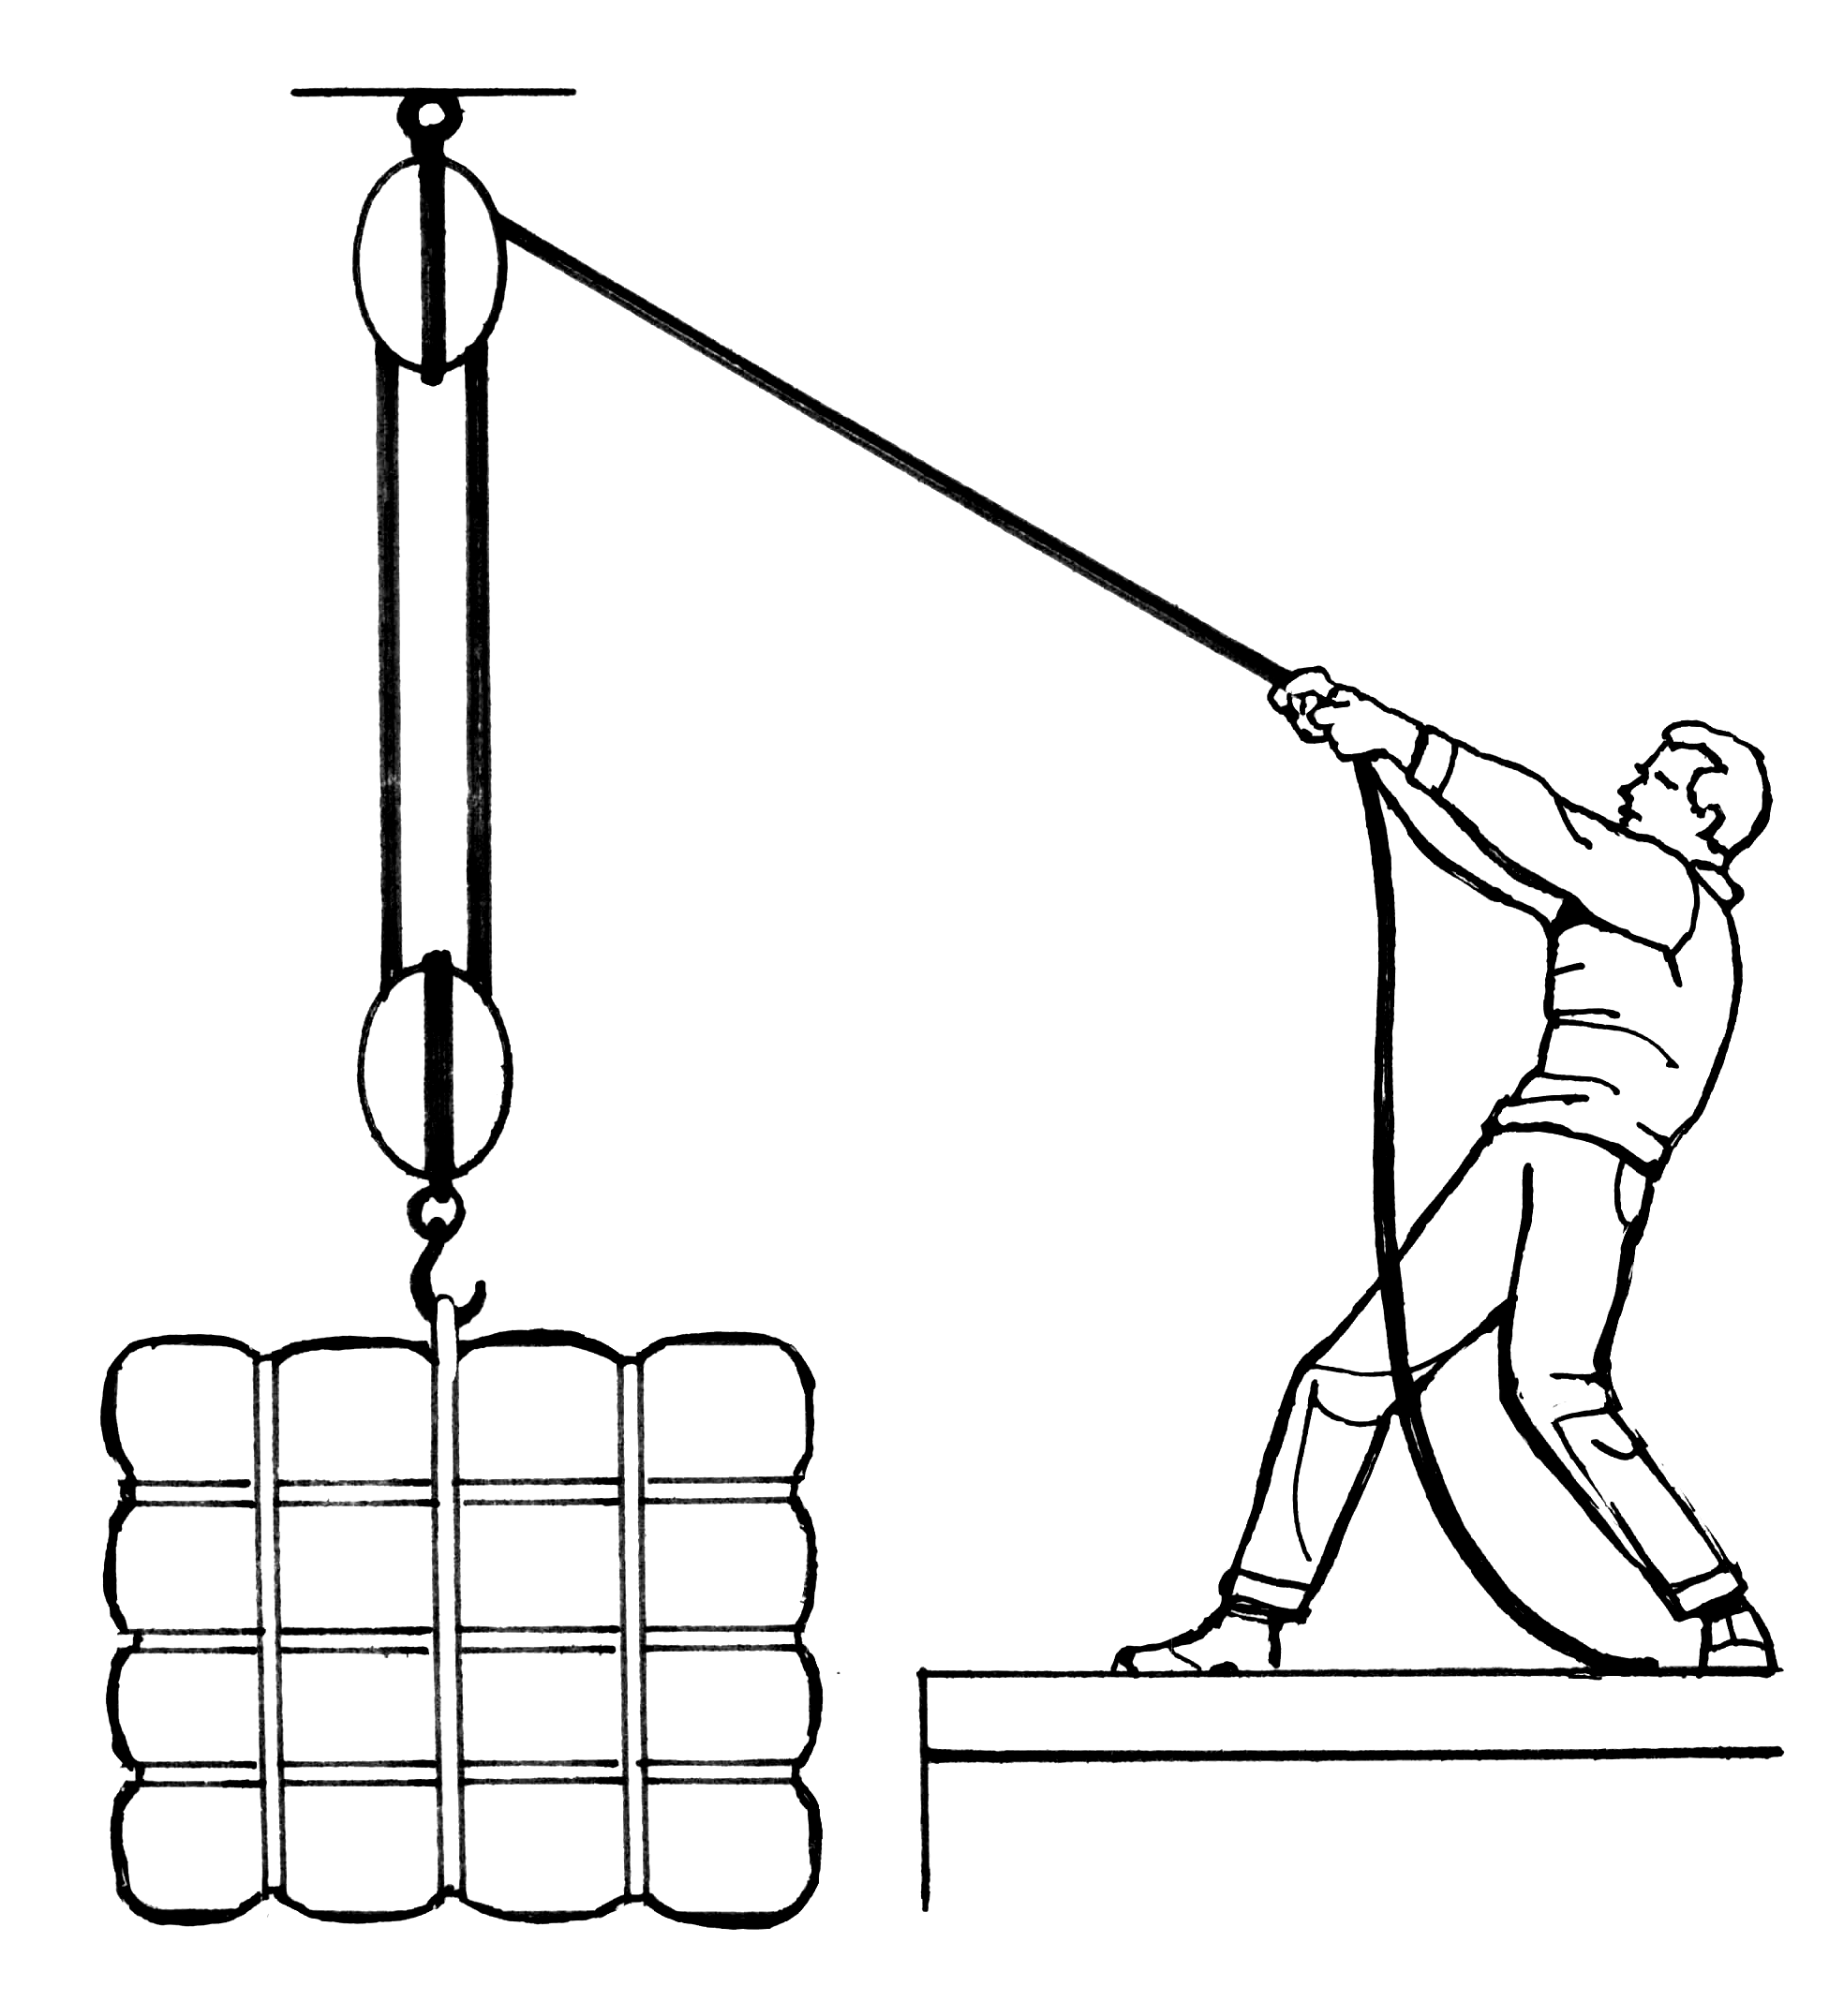
\includegraphics[width=0.3\textwidth]{blockandtackle.png}

       Suppose the load has a weight of 1250 N. 

       \begin{enumerate}
         \item{Suppose our person lifts this load two meters slowly (at constant velocity). What force must he exert on the rope to do so?} 
         \item{It seems like he's getting something for nothing -- that he's able to lift a larger weight with a smaller force. But is he? Calculate the work done by the rope on the load, and calculate the work he does on the rope.}
         \item{If he lifts this load 2m and then holds it there, clearly its change in kinetic energy is zero: it started at rest and ended at rest. However, the rope did positive work on the load; the work-energy theorem thus says that its kinetic energy should
             increase unless some other force did an equal amount of negative work on it. What force was this?}
         \item{Explain why, using the definition of work $W = \int \vec F \cdot d\vec s$, that force does negative work.}
       \end{enumerate}
     }

   \item{{\it (The following problem is extra credit.)} At high speed, the main retarding force on an automobile is air drag. We haven't specifically studied air drag yet, 
but it's quite simple. The drag force is very well approximated as 

      \begin{equation*}
        F_{\rm {drag}} = \gamma v^2
      \end{equation*}

      where $\gamma$ depends on the shape and size of the car. 

      Consider a car with $\gamma = 1.9 \, \rm N / \left(\frac{\rm m}{\rm s}\right)^2$ and an engine that develops a maximum power of 75 kW. (Remember, this means that the engine does 75 kJ of work per second.) These are rough estimates of the parameters of a small sedan.

      \begin{enumerate}
        \item{What is the maximum speed of this car, in miles (or km) per hour? Note that the maximum speed is
the speed where the rate at which the engine does positive work on the car is the same as the rate at which 
air drag does negative work. Recall that if work equals force times distance, I can take the time derivative 
of both sides to get $P=\vec F \cdot \vec v$.}
        \item{Suppose that, rather than driving at its maximum speed, the driver travels only at 100 km/hr. What power is required from the engine to go this fast?}
        \item{It's said that one of the most important things a driver can do to save fuel is to slow down. Suppose a given trip requires 10 gallons of gas at 70 miles per hour. How much gas will it require at 60 miles per hour?\\
          {\sc Note:} If you wind up doing a great many unit conversions for this problem, you're making it far harder than it should be. The easiest approach here is to figure out the energy required for a trip as a function of distance and speed,
        and then see how it depends on the speed. You can use dimensional analysis to very quickly see if your formula is correct.}
    \end{enumerate}
  }




    \end{enumerate}

\end{document}
